\chapter{Operationen}

\section{Suchen}

Um einen Schl\"ussel innerhalb eines B-Baums zu suchen geht man folgenderma\ss{}en vor. Ausgehend von der Wurzel werden alle Knoten danach \"uberpr\"uft, ob sich der Schl\"ussel in dem betrachteten Knoten befindet. Wird er nicht in der Wurzel gefunden wird der kleinste Schl\"ussel, der gr\"o\ss{}er als der gesuchte Schl\"ussel ist bestimmt. Sofern dieser Schl\"ussel existiert, wird bei dem Kindknoten links von diesem weitergesucht. Wenn die Suche am Ende bei einer null-Referenz landet existiert der Schl\"ussel nicht, oder er wurde nicht gefunden.
\\[0.5in]
\begin{figure}[h!] %[hbtp]
	\centering
	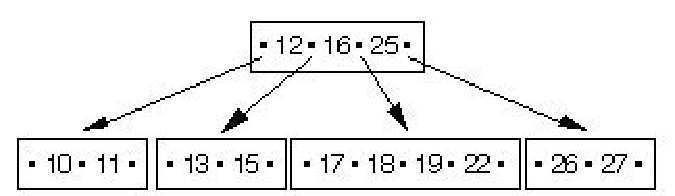
\includegraphics[width=0.7\linewidth]{images/Beispiel_Suche_B-Baum.pdf}
	\caption{Beispiel B-Baum}
	\label{Beispiel_Suche_B-Baum}
\end{figure}
\\[0.3in]
\section{Einf\"ugen}
Damit ein neuer Knoten eingef\"ugt werden kann, wird zuerst das Blatt bestimmt in dem sich der Schl\"ussel befinden m\"usste. Daher es den Schl\"ussel noch nicht gibt, bleibt die Suche erfolglos. Nun k\"onnen 2 F\"alle eintreten, wie der neue Schl\"ussel in den B-Baum eingef\"ugt werden kann. Hierbei ist zu beachten, dass nur $m-1$ Schl\"ussel pro Knoten gespeichert werden k\"onnen. 
\paragraph{Fall 1.}
Der Knoten k hat m-1 Schl\"ussel noch nicht gespeichert und es wurde der Schl\"ussel $x$ auch in der Blattebene nicht gefunden, so wird der Schl\"ussel in den B-Baum eingef\"ugt. In diesem Fall f\"ugt man den Schl\"ussel $x$ in dem Knoten $k$ zwischen $x_{i}$ und $ x_{i+1} $ ein.
\newline
Ein Beispiel:
\newline
Wir f\"ugen in (siehe Abb. \ref{Beispiel_Suche_B-Baum})  den Schl\"ussel 14 ein. Zuerst beginnt der Suchbaum in der Wurzel $-12-16-$($12<14>16$), der Schl\"ussel wechselt in den Kindknoten zwischen 12 und 16. Dieser Knoten besitzt die Schl\"ussel $-13-15-$. Daher der B-Baum die Ordnung $m=5$ besitzt, ist in dem Knoten noch Platz f\"ur einen weiteren Schl\"ussel. Dort wird der Schl\"ussel nach der Definition (siehe Kapitel \ref{def}) eingef\"ugt.(siehe Abb. \ref{insert_01}) 
\\[0.5in]
\begin{figure}[h!] %[hbtp]	
\centering
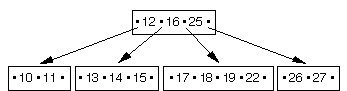
\includegraphics[width=0.7\linewidth]{images/insert_01}
\caption{14 einf\"ugen}
\label{insert_01}
\end{figure}
\\[0.3in]
\paragraph{Fall 2:}
Es wurden bereits $m-1$ Schl\"ussel in dem Knoten gespeichert, zudem der Schl\"ussel $x$ geh\"oren w\"urde. Der Schl\"ussel wird daher zuerst in den betreffenden Knoten seiner Gr\"o\ss{}e nach eingef\"ugt und der zu gro\ss{}e Knoten in der Mitte geteilt. Der mittlere Knoten wandert in seinen Vaterknoten und ordnet sich dort seiner Gr\"o\ss{}e nach ein. Die Zeiger auf die Kindknoten passen sich der neuen Anordnung an.
\newline
Ein Beispiel:
\newline
In die vorherige Abbildung (siehe Abb. \ref{insert_01}) wird der neue Schl\"ussel $24$ eingef\"ugt. Daher der Knoten zu gro\ss{} wird, teilt er sich und der Schl\"ussel $19$ wandert in den Vaterknoten. Danach bilden sich 2 neue Knoten aus dem zu gross{}en Knoten.(siehe Abb. \ref{insert_02})
\\[0.5in]
\begin{figure}[h!] %[hbtp]	
	\centering
	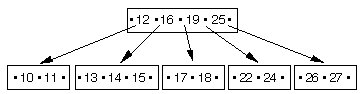
\includegraphics[width=0.7\linewidth]{images/insert_02}
	\caption{24 einf\"ugen}
	\label{insert_02}
\end{figure}
\newpage
\section{L\"oschen}
L\"oschen in B-B\"aumen ist im Gegenzug zu anderen B\"aumen komplexer, da sehr genau zwischen dem L\"oschen von Knoten und von Bl\"attern unterschieden werden muss.
Hierbei kann man 3 F\"alle unterscheiden.
\begin{enumerate}
	\item Wenn das Blatt die Wurzel ist und das Blatt leer ist kann die Wurzel gel\"oscht werden. Der Baum ist leer.
	\item Wenn das Blatt nicht die Wurzel ist, und  $m\geq \lceil n/2\rceil-1$ Schl\"ussel besitzt. Dann ist das L\"oschen beendet.
	\item Wenn jedoch $m= \lceil n/2\rceil-2$, so muss die Eigenschaft des B-Baums wiederhergestellt werden.
		\begin{enumerate}
				\item Gibt es einen Nachbarn, der $m> \lceil n/2\rceil-1$, so k\"onnen Schl\"ussel zwischen den beiden Knoten verschoben werden.
				\item Gilt f\"ur beide Knoten jedoch, $m= \lceil n/2\rceil-1$, so m\"ussen 2 Knoten vereinigt werden.
		\end{enumerate}	
\end{enumerate}

\paragraph{Verschiebung von Schl\"usseln beim L\"oschen} 
\begin{tabular}{|l|l|}
	\hline Nur rechter Nachbar vorhanden mit\\ $m_{rechts}> \lceil n/2\rceil -1$  & Linksverschiebung  \\ 
	\hline Linker und rechter Nachbar vorhanden mit\\ $m_{links>}> \lceil n/2\rceil -1$ und $m_{rechts>}> \lceil n/2\rceil -1$ und $ m_{links} m_{rechts}$ & Linksverschiebung \\ 
	\hline Linker und rechter Nachbar vorhanden mit\\ $m_{links>}> \lceil n/2\rceil -1$ und $m_{rechts>}> \lceil n/2\rceil -1$ und $ m_{links} m_{rechts}$ & Rechtsverschiebung \\ 
	\hline nur linker Nachbar vorhanden mit\\ $m_{rechts}> \lceil n/2\rceil -1$ & Rechtsverschiebung \\ 
	\hline 
\end{tabular} 
\paragraph{Vereinigung von Knoten beim L\"oschen} 

Vereinigung mit rechtem Nachbarn nach L\"oschen von a3(siehe Abb. \ref{loeschen_01})
\begin{figure}[h!] %[hbtp]	
	\centering
	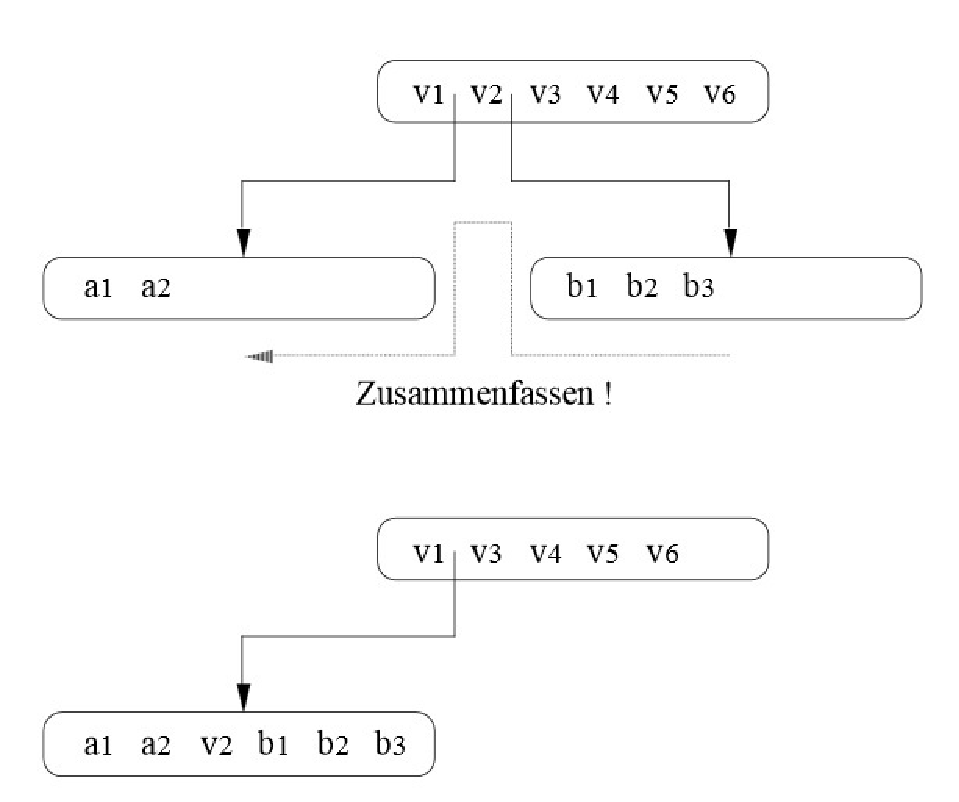
\includegraphics[width=0.7\linewidth]{images/loeschen_01}
	\caption{}
	\label{loeschen_01}
\end{figure}
\newpage
\begin{itemize}
	\item Durch das Vereinigen von Knoten wird die Zahl der Werte m im Vorg\"angerknoten um eins kleiner.
	\item Daher kann dort wiederum ein Unterschreiten der Untergrenze stattfinden.
	\item Vereinigungsvorg\"ange k\"onnen sich daher bis zur Wurzel fortsetzen.
	\item ie Wurzel selbst darf jedoch weniger als $\lceil n/2\rceil -1$ Werte besitzen, so dass hier der Vorgang endet
	
\end{itemize}